\part{SW 11}
\section{Lernziele (Leitfragen)}
\begin{enumerate}
    \item Was sind typische Informationssicherheitsziele?
    \item Wozu braucht man Netzwerksicherheit?
    \item Was ist eine Bedrohung (Threat)?
    \item Was ist ein Asset?
    \item Was ist eine Schwachstelle (Vulnerability)?
    \item Was ist Risiko (im Kontext der Informationssicherheit)?
    \item Was ist ein "`mitigation technique"'?
    \item Wieso ist es so schwierig völlig sichere Systeme zu erstellen?
    \item Was ist Vertraulichkeit und wie ist sie normalerweise (technisch) erreicht?
    \item Was ist Integrität und wie ist sie normalerweise (technisch) erreicht?
    \item Was ist Verfügbarkeit und wie ist sie normalerweise (technisch) erreicht?
    \item Was ist Authentifizierung und wie ist sie normalerweise (technisch) erreicht?
    \item Was ist "`non-repudiation"' und wie ist es normalerweise (technisch) erreicht?
    \item Was ist der Unterschied zwischen symmetrischer und asymmetrischer Kryptografie?
    \item Welche Kryptografieart (symmetrisch oder asymmetrisch) wird für digitale Unterschriften verwendet?
    \item Geben Sie ein Beispiel eines symmetrischen kryptografischen Algorithmus
    \item Geben Sie ein Beispiel eines asymmetrischen kryptografischen Algorithmus
\end{enumerate}

\section{Antworten}
{\color{teal}\textsf{\textbf{Anmerkung: viel Text wurde aus meiner eigenen ISF Zusammenfassung auf \\\url{https://github.com/vigi86/HSLU_Zusammenfassungen} entnommen. Das Fach "`Information Security Fundamentals"' behandelt, wer hätte es gedacht, Informationssicherheit.}}}

\subsection*{Was sind typische Informationssicherheitsziele?}\label{sub:Informationssicherheitsziele}
Es gibt Basis- und erweiterte Ziele. Basisziele sind \textbf{Verfügbarkeit, Integrität, Verbindlichkeit und Vertraulichkeit}.
\paragraph*{Verfügbarkeit}\label{par:Availability}\index{Grundziele Informationssicherheit}\index{Schutzziele}\index{Informationssicherheitsziele}
\begin{itemize}
    \item \textbf{Verfügbarkeit} ist gewährleistet, wenn in der vom Benutzer gewünschten Zeit auf Dienste oder Informationen zugegriffen werden kann (Ausfallquote)
    \item Engl.: \textbf{Availability}
\end{itemize}

\paragraph*{Integrität}\label{par:Integrity}\index{Integrität}
\begin{itemize}
    \item \textbf{Integrität} ist gewährleistet, wenn Daten oder Systeme nicht unautorisiert oder zufällig manipuliert oder verändert werden können (Datensicherheit)
    \item Engl.: \textbf{Integrity}
\end{itemize}
\begin{figure}[H]
    \begin{center}
    \label{pic:Hash}
    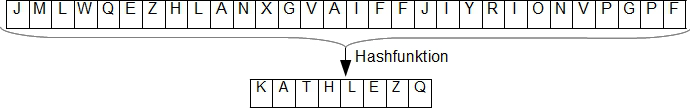
\includegraphics[width=\textwidth]{images/hash.png}
    \caption{Hashfunktion (Quelle: ISF Folien, Prof. Dr. Hänggi)}
    \end{center}
\end{figure}

\pagebreak
\paragraph*{Verbindlichkeit}\label{par:Non-Repudiation}\index{Verbindlichkeit}
\begin{itemize}
    \item \textbf{Verbindlichkeit}liegt vor, wenn eine Handlung eindeutig einer Person zugeordnet und von dieser nicht geleugnet werden kann
    \item Engl.: \textbf{Non-Repudiation}
\end{itemize}
\begin{figure}[H]
    \begin{center}
    \label{pic:Signature}
    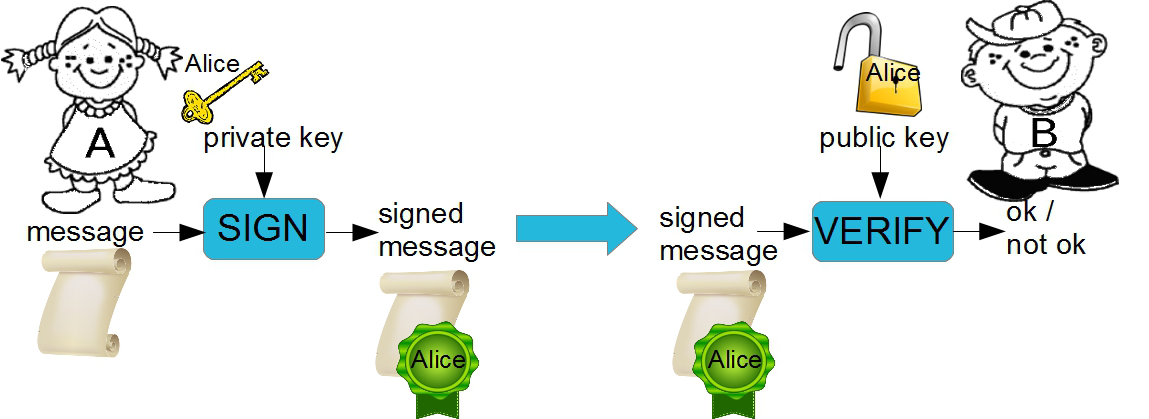
\includegraphics[width=.9\textwidth]{images/sign1.png}
    \caption{Identitätsbeweis mittels Signatur (Quelle: ISF Folien, Prof. Dr. Hänggi)}
    \end{center}
\end{figure}

\paragraph*{Vertraulichkeit}\label{par:Confidentiality}\index{Vertraulichkeit}
\begin{itemize}
    \item \textbf{Vertraulichkeit} ist gegeben, wenn sichergestellt werden kann, dass Informationen nicht durch unautorisierte Personen, Instanzen oder Prozesse eingesehen werden können
    \item Engl.: \textbf{Confidentiality}
\end{itemize}
\begin{figure}[H]
    \begin{center}
    \label{pic:SymmetricEncryption}
    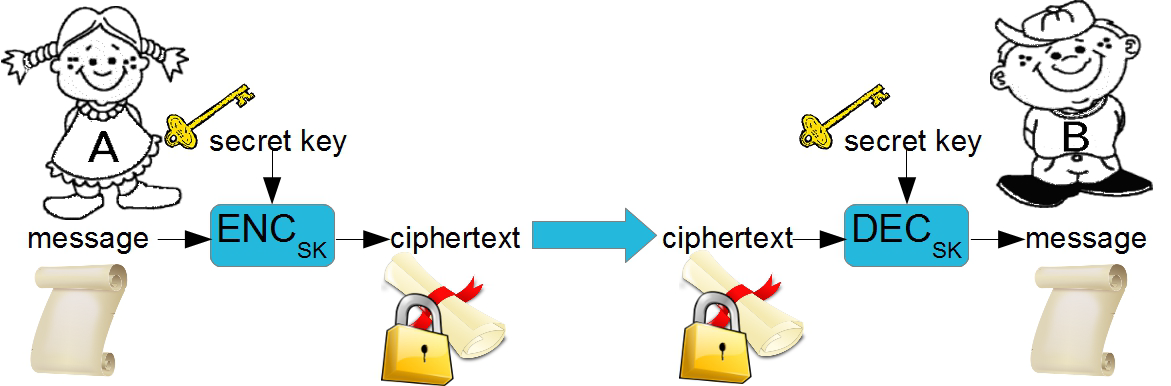
\includegraphics[width=.9\textwidth]{images/secretkey.png}
    \caption{Symmetrisches Verschlüsselungsverfahren (Quelle: ISF Folien, Prof. Dr. Hänggi)}
    \end{center}
\end{figure}
\begin{figure}[H]
    \begin{center}
    \label{pic:AsymmetricEncryption}
    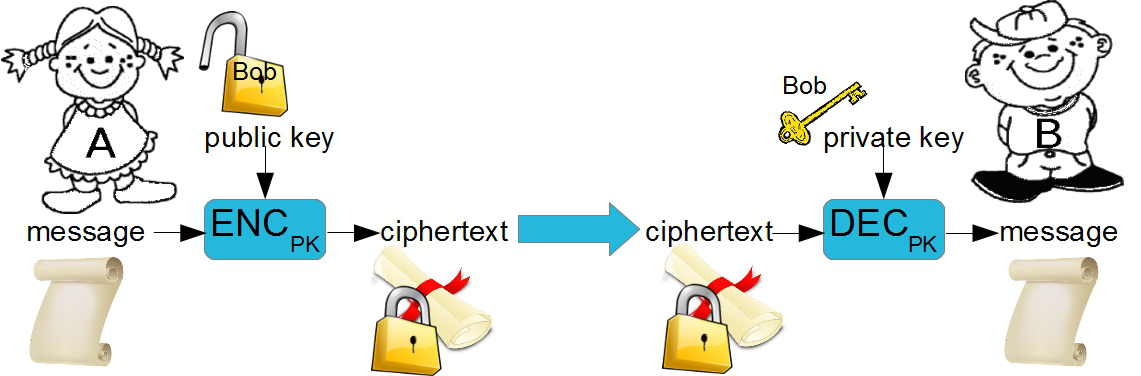
\includegraphics[width=.9\textwidth]{images/publickey.png}
    \caption{Asymmetrisches Verschlüsselungsverfahren (Quelle: ISF Folien, Prof. Dr. Hänggi)}
    \end{center}
\end{figure}

\pagebreak
\paragraph*{Identität / Authentizität}\label{par:IdentityAuthenticity}\index{Identität}\index{Authentizität}
\begin{itemize}
    \item \textbf{Identität:} "`Beim Menschen bezeichnet Identität die ihn kennzeichnende und als Individuum von anderen Menschen unterscheidende Eigentümlichkeit seines Wesens."'\cite{wiki} Informationstechnische Anwendungen: Fingerabdruck, Iris, Handvenen.
    \item \textbf{Authentizität:} "`In der Informationssicherheit bezeichnet Authentizität die Eigenschaften der Echtheit, Überprüfbarkeit und Vertrauenswürdigkeit. Die Überprüfung einer behaupteten Eigenschaft wird als Authentifikation bezeichnet. Durch Authentifikation des Datenursprungs wird nachgewiesen, dass Daten einem angegebenen Sender zugeordnet werden können, was durch digitale Signaturen ermöglicht werden kann."'\cite{wiki} Informationstechnische Anwendung:
    \item[$\rightarrow$] Siehe unten Authentisierung, Authentifizierung und Autorisierung.
\end{itemize}

\paragraph*{Wichtige Grundbegriffe sind}\textbf{Zutritts-, Zugangs-, Zugriffskontrolle}
\begin{itemize}
    \item \textbf{\textsl{Zutrittskontrolle: }}Schutz des physischen Systems (Bsp. Serverraum, Schlüssel)\index{Zutrittskontrolle}
    \item \textbf{\textsl{Zugangskontrolle: }}Schutz des logischen Systems (Bsp. Betriebssystem, Login)\index{Zugangskontrolle}
    \item \textbf{\textsl{Zugriffskontrolle: }}Daten-bezogen; Schutz der Operationen (Bsp. Dateisystem, Benutzerrechte)\index{Zugriffskontrolle}
\end{itemize}

\subsubsection*{Begriffe}Bei der Zugriffskontrolle unterscheidet man drei Begriffe: Authentisierung, Authentifizierung und Autorisierung.

\paragraph*{Authentisierung}\label{par:Authentication}\index{Authentisierung}\label{para:Authentisierung}Die Authentisierung ist ein \textbf{Nachweis einer Person}, dass sie tatsächlich die Person ist, die sie vorgibt zu sein.
\begin{itemize}
    \item geheime Information, dass nur ihr bekannt ist (Passwort)
    \item Identifizierungsgegenstand (z.B. Identitätskarte)
    \item sie ist selbst das Identifizierungsobjekt (z.B. Fingerabdruck)
\end{itemize}

\subparagraph*{Methoden der Authentisierung}\index{Authentisierung}
\begin{itemize}
    \item Etwas, das ich weiss (\textbf{Wissen})
    \begin{itemize}
        \item Passwort
        \item Pin
        \item Sicherheits- / Geheimfragen
    \end{itemize}
    \item Etwas, das ich habe (\textbf{Besitz})
    \begin{itemize}
        \item Physikalischer Schlüssel
        \item Magnetstreifenkarte
        \item Hardware-Token\footnote{z.B. Kartenleser für E-Banking}
    \end{itemize}
    \item Etwas, das ich bin (\textbf{Eigenschaft} / körperliches Merkmal)
    \begin{itemize}
        \item Foto
        \item Fingerabdruck
        \item Iris
    \end{itemize}
    \item Etwas, das ich kann (\textbf{Fähigkeit})
    \begin{itemize}
        \item Unterschrift
        \item Stimmenerkennung (Sprechen)
    \end{itemize}
\end{itemize}

\subsubsection*{Wissen}
Vorteil
\begin{itemize}
    \item man benötigt keine zusätzlichen Hilfsmittel
\end{itemize}
Nachteil
\begin{itemize}
    \item kann vergessen oder (v)erraten werden (Passwort, Geheimfragen)
\end{itemize}

\subsubsection*{Besitz}
Vorteil
\begin{itemize}
    \item kann benutzerindividuelle Daten speichern
    \item kann sich selbst schützen und aktiv verändern (SecurID, Smartcard)
\end{itemize}
Nachteil
\begin{itemize}
    \item Verwaltung des Besitzes ist unsicher und muss mitgeführt werden
    \item kann verloren gehen (Schlüssel, Karte, HW-Token)
\end{itemize}

\subsubsection*{Eigenschaft / körperliches Merkmal}
Vorteil
\begin{itemize}
    \item kann nicht verloren werden
    \item kann nicht an Dritte weitergegeben werden
\end{itemize}
Nachteil
\begin{itemize}
    \item benötigt zur Erkennung spezielle Vorrichtung (Technik)
    \item fälschliche Akzeptanz/Zurückweisung möglich
\end{itemize}

\subsubsection*{Fähigkeit}
Vorteil
\begin{itemize}
    \item ziemlich einmalig, schwierig zu kopieren
\end{itemize}
Nachteil
\begin{itemize}
    \item kann von Nachahmern imitiert werden
    \item kann Probleme beim Datenschutz aufwerfen
\end{itemize}

\paragraph*{Authentifizierung}\label{par:Authentification}\index{Authentifizierung}\label{para:Authentifizierung}Die Authentifizierung ist die \textbf{Prüfung der behaupteten Authentisierung}. Die Authentifizierung wird von einem \textbf{Prüfer} durchgeführt. Der Prüfer überprüft die Echtheit der Authentisierung.
\begin{figure}[H]
    \begin{center}
    \label{pic:HMAC}
    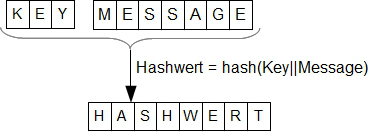
\includegraphics[width=\textwidth]{images/hmac.png}
    \caption{Erstellen eines HMAC}
    \end{center}
\end{figure}

\paragraph*{Autorisierung}\label{par:Authorization}\index{Autorisierung}\label{para:Autorisierung}Die Autorisierung räumt Rechte für die Nutzung von speziellen Diensten und Leistungen ein.

\subsection*{Wozu braucht man Netzwerksicherheit?}
Um Informationen zu sichern. Es sollte sichergestellt werden, dass niemand auf Informationen zugreifen oder verändern kann, die er nicht dürfte.

\subsection*{Was ist eine Bedrohung (Threat)?}
\begin{itemize}
    \item Ein Threat hat mit Folgen zu tun (wirtschaftlicher Schaden)
    \item Angreifer bewegen sich in einem "`Attack Vector"', einem angreifbarem Bereich. Etwas, das Schwachstellen aufweist.
    \item Beispiele
    \begin{itemize}
        \item Informationsdiebstahl
        \item Datenverlust
        \item Datenmanipulation
        \item Disruption of Service (Betriebsstörung)
        \item VERLUST VON ZEIT UND GELD
    \end{itemize}
\end{itemize}

\paragraph*{Was gefährdet die Informationen?} Welche Gefährdungen/Bedrohungen gibt es?\index{Gefährdungen}\index{Bedrohungen}\index{Informationssicherheit}
\begin{itemize}
    \item Nicht vorsätzliche (zufällige) Gefährdungen/Bedrohungen
    \begin{itemize}
        \item Naturgewalten (Blitz, Hagel, Unwetter, Erdrutsche, Hochwasser, etc.)
        \item Ausfall von Strom oder Telekommunikation
        \item Technische Pannen, z.B. Fehler von Hard- und/oder Software
        \item Bedienerfehler / Fahrlässigkeit der Mitarbeitenden
    \end{itemize}
    \item Vorsätzliche Gefährdungen/Bedrohungen
    \begin{itemize}
        \item Bösartiger Code (Viren, Würmer, Trojaner, etc.)
        \item Informationsdiebstahl
        \item Angriffe (von Skript-Kiddies bis Hacker)
        \item Wirtschaftsspionage ("`was die Konkurrenz wissen möchte"')
        \item Missbrauch der IT-Infrastruktur
    \end{itemize}
\end{itemize}

\paragraph*{Menschliches Fehlverhalten}durch Fahrlässigkeit, Gleichgültigkeit, Unwissenheit und Leichtgläubigkeit.


\paragraph*{Vorsätzliche Manipulation}
\begin{itemize}
    \item Angriffe über das Internet
    \item Unerlaubter Zugriff auf Systeme
    \item Abhören und Modifizieren von Daten
    \item Angriff auf die Verfügbarkeit von Systemen
    \item Missbrauch von Systemen, Distributed Denial of Service (DDoS)\index{DDoS}
    \item Viren, Würmer und Trojanische Pferde
    \item Drive by Infection\footnote{unbeabsichtigtes Downloaden von Schadsoftware}
\end{itemize}

\paragraph*{Organisatorische Schwachstellen}
\begin{itemize}
    \item Fehlendes Sicherheitsverständnis des Managements
    \item Unklare Verantwortlichkeiten
    \item Ungenaue oder fehlende Abläufe / Prozesse
    \item Mangelhafte Richtlinien
    \item Fehlende Strategie und Konzepte
    \item Mangelhafte Awareness der Mitarbeitenden
    \item Fehlende Kontrollen
\end{itemize}

\paragraph*{Technisches Versagen}
\begin{itemize}
    \item Ungenügende Wartung
    \item Nicht funktionierende Überwachungssysteme (z.B. IDS\footnote{Intrusion Detection System}, etc.)
    \item Falsch dimensionierte Systeme
    \item Fehlerhafte
    \begin{itemize}
        \item Konfiguration
        \item Applikationen
        \item Betriebssysteme
        \item Firmware
        \item Treiber
    \end{itemize}
\end{itemize}

\paragraph*{Höhere Gewalt}
\begin{itemize}
    \item Ökologisch
    \begin{itemize}
        \item Unwetter
        \item Erdbeben
        \item Brände
        \item Überschwemmungen
    \end{itemize}
    \item Technisch
    \begin{itemize}
        \item Feuer
        \item Wasser
    \end{itemize}
    \item Sozial
    \begin{itemize}
        \item Ausschreitungen
        \item Geiselnahme
        \item Krieg
    \end{itemize}
\end{itemize}

\subsection*{Was ist ein Asset?}
\begin{itemize}
    \item z.B. Computer = kostet etwas, hat einen Wert
    \item hat eine Wichtigkeit
    \item Kundendaten sind wichtig und aus der Sicht der Firma wertvoll uns sind ein Asset
\end{itemize}

\subsection*{Was ist eine Schwachstelle (Vulnerability)?}
Schwachstellen sind Stellen, die für Angriffe anfällig sind. Man beachtet dabei das Mass einer Schwachstelle in einem Netzwerk oder Gerät. Schwachstellen sind inhärent\footnote{"`Innewohnen"'} und unvermeidbar in Netzwerk- und Endgeräten. Sogar in Geräten mit Sicherheitseinrichtung.

\subsection*{Was ist Risiko (im Kontext der Informationssicherheit)?}
\paragraph*{Risiko}\index{Risiko}\label{para:Risiko}Ein Risiko ist ein negativer Ausgang einer Unternehmung, mit dem Nachteile, Verlust, Schäden, usw. verbunden sind.
\begin{itemize}
    \item Wahrscheinlichkeit, dass eine Gefährdung über eine Schwachstelle zu einem Schaden von bestimmten Ausmass führt
    \item Wahrscheinlichkeiten sind extrem schwer zu berechnen $\rightarrow$ Geschätzte Häufigkeiten
    \item \textbf{Risiko = Eintretenshäufigkeit $\times$ Schadensausmass}
    \item Die Eintretenshäufigkeit und Schaden können bewertet werden
    \item Sicherheit und Risiko sind voneinander abhängig
\end{itemize}

\subsection*{Was ist ein "`mitigation technique"'?}
Eine Art ein Risiko zu behandeln. Nicht jedes Risiko muss aber aber abgedeckt, bzw. geschützt werden. Es gibt auch akzeptable Risikos, bei dem beispielsweise die Kosten den Nutzen übersteigen. Die Mitigation an sich ist es mit geeigneten Sicherheitsmassnahmen das Schadensausmass oder die Eintrittshäufigkeit reduzieren.

\subsection*{Wieso ist es so schwierig völlig sichere Systeme zu erstellen?}
Systeme werden immer komplexer und diese verbergen eher Schwachstellen. Cloudsysteme sind beispielsweise komplexe Strukturen und machen die Anwendung von Sicherheitsmechanismen schwierig.

\subsection*{Was ist Vertraulichkeit und wie ist sie normalerweise (technisch) erreicht?}
Durch Verschlüsselung. Siehe vorhin \underline{\nameref{par:Confidentiality}}, Seite \pageref{par:Confidentiality}.

\subsection*{Was ist Integrität und wie ist sie normalerweise (technisch) erreicht?}
Mit Hashfunktionen. Die kleinste Änderung am Daten-Input gibt einen ganz anderen Hash-Output. Ein gleicher Daten-Input gibt aber immer denselben Hash-Output. Siehe vorhin \underline{\nameref{par:Integrity}}, Seite \pageref{par:Integrity}.

\subsection*{Was ist Verfügbarkeit und wie ist sie normalerweise (technisch) erreicht?}
Viel \textbf{virtualisieren}, damit Services eine hohe Verfügbarkeit bieten. Wenn mehr \textbf{Kapazität} (z.B. Daten- oder Arbeitsspeicher) notwendig ist, kann rasch mehr hinzugefügt werden. \textbf{Proxies} verhinder, dass viele Verbindungen zum Server von der gleichen IP hergestellt werden können. Siehe vorhin \underline{\nameref{par:Availability}}, Seite \pageref{par:Availability}.

\subsection*{Was ist Authentifizierung und wie ist sie normalerweise (technisch) erreicht?}
\textbf{Authentifizierung} ist ein Prozess, bei dem zuletzt eine \textbf{Authentisierung} durchgeführt wird. Eine Prüfnachricht, welche von einem Prüfer (Server, Remote Client etc.) erhalten wurde, wird zusammen mit einem Secret Key (Passwort) clientseitig gehasht. Dieser erzeugte Hash ist ein sogenannter HMAC - Hashed Message Authentication Code. Der HMAC wird zurück an den Prüfer gesendet. Dieser kann eine \textbf{Authentisierung} vornehmen und deren Echtheit prüfen. Dieser Vorgang läuft im Hintergrund ab, beispielsweise wenn man sich auf einer Webseite einloggt. In Englisch gibt es lexikalisch keine Unterscheidung, es heisst beides \textsl{Authentication}. Siehe vorhin \underline{\nameref{par:Authentification}}, Seite \pageref{par:Authentification} und \underline{\nameref{par:Authentication}}, Seite \pageref{par:Authentication}.

\subsection*{Was ist "`non-repudiation"' und wie ist es normalerweise (technisch) erreicht?}
Verbindlichkeit erzielt man mittels digitaler Signatur. Wenn ich beispielsweise jemanden eine Email sende, signiere ich die Email mit meinem privaten Schlüssel, den nur ich besitze. Der Empfänger kennt hingegen meinen öffentlichen Schlüssel und nutzt diesen, um sich zu vergewissern, dass die Email tatsächlich von mir gesendet wurde. Siehe vorhin \underline{\nameref{par:Non-Repudiation}}, Seite \pageref{par:Non-Repudiation}.

\subsection*{Was ist der Unterschied zwischen symmetrischer und asymmetrischer Kryptografie?}
\begin{itemize}
    \item Symmetrisch: verwendet einen einzigen Schlüssel. Alle Parteien besitzen denselben Schlüssel.
    \item Asymmetrisch: Jede Partei besitzt einen öffentlichen und einen privaten Schlüssel (public/private key). Der öffentliche Schlüssel ist für alle verfügbar. Zum verschlüsseln braucht man den öffentlichen Schlüssel des Empfängers. Der Empfänger kann mittels seinem privaten Schlüssel die Nachricht oder Dateien entschlüsseln.
\end{itemize}
Siehe vorhin \underline{\nameref{par:Confidentiality}}, Seite \pageref{par:Confidentiality}.

\subsection*{Welche Kryptografieart (symmetrisch oder asymmetrisch) wird für digitale Unterschriften verwendet?}
Asymmetrisch. Siehe vorhin \underline{\nameref{par:Non-Repudiation}}, Seite \pageref{par:Non-Repudiation}.

\subsection*{Geben Sie ein Beispiel eines symmetrischen kryptografischen Algorithmus}\index{Algorithmen!symmetrisch}
Beispiele für symmetrische Algorithmen\\
\begin{tabular}{|c|c|c|c|c|}
    \hline
    Name&Blocklänge&Schlüssellänge&Jahr&Kommentar\\
    \hline
    DES&64 Bit&56 Bit&1970&gebrochen\\
    Triple DES&64 Bit&112 Bit ($3\times56$ Bit)&  &nicht mehr empfohlen\\
    RC4&stream cipher&8-2040&1987&gebrochen\\
    IDEA&64 Bit&128 Bit&1990&nicht mehr empfohlen\\
    RC5&64 oder 128 Bit&4-256 Bit&1994&nicht mehr empfohlen\\
    Camellia&128 Bit&128, 192 oder 256 Bit&2000& \\
    Twofish&128 Bit&128, 192 oder 256 Bit&1998& \\
    AES (Rijndal)&128 Bit&128, 192 oder 256 Bit&2000& \\
    \hline
\end{tabular}

\subsection*{Geben Sie ein Beispiel eines asymmetrischen kryptografischen Algorithmus}\index{Algorithmen!asymmetrisch}
Beispiele für asymmetrische Algorithmen\\
\begin{tabular}{|c|c|}
    \hline
        Name&Unterliegende `schwierige' Funktion\\
        \hline
        RSA&Faktorisieren grosser Zahlen\\
        Diffie-Hellman (DH)&Diskrete Logarithmen berechnen\\
        Elliptic Curve DH (ECDH) &Diskrete Logarithmen berechnen\\
        ElGamal Verschlüsselung&Diskrete Logarithmen berechnen\\
    \hline
\end{tabular}
